\documentclass[10pt]{article}
\usepackage[utf8]{inputenc}\usepackage[T1]{fontenc}\usepackage[spanish,es-nodecimaldot]{babel}
\usepackage[margin=1.9cm]{geometry}\usepackage{graphicx,booktabs,amsmath,hyperref,xcolor,float,titlesec,enumitem}
\definecolor{acc}{HTML}{C2410C}
\titleformat{\section}{\large\bfseries\color{acc}}{\thesection}{0.5em}{}\titlespacing*{\section}{0pt}{9pt}{3pt}
\setlist{nosep,leftmargin=1.2em}\setlength{\parskip}{3pt}\setlength{\parindent}{0pt}
\hypersetup{colorlinks=true,urlcolor=blue!50!black}\emergencystretch=3em\sloppy
\begin{document}
\begin{center}{\LARGE\bfseries Informe final. Sequ\'ia en el Corredor Seco con GPU}\\[3pt]
Caso 4, Agricultura y clima \textperiodcentered{} CC3069 Computaci\'on Paralela y Distribuida, Secci\'on 20 \textperiodcentered{} Universidad del Valle de Guatemala \textperiodcentered{} 11 de noviembre de 2026\\[3pt]
Javier Eduardo Espa\~na Pacheco (23361) \textperiodcentered{} Angel Esteban Esquit Hern\'andez (23221) \textperiodcentered{} Jos\'e Antonio M\'erida Castej\'on (201105)\end{center}

\section{Problema e impacto esperado}
Las familias campesinas del Corredor Seco (Zacapa, Chiquimula, El Progreso, Jalapa, Jutiapa y Baja Verapaz) dependen de una sola cosecha de ma\'iz y frijol al a\~no. El MAGA necesita avisarles antes de que la sequ\'ia arruine la cosecha, para que puedan sembrar semilla resistente, mover la fecha de siembra o pedir ayuda alimentaria. Si calcular el \'indice de lluvia de toda la regi\'on tarda horas o d\'ias, la alerta llega tarde. Si tarda segundos, se puede recalcular con cada dato nuevo y probar distintas definiciones de sequ\'ia.

\section{Datos, tama\~no, limpieza y preparaci\'on}
\textbf{Fuente.} Rean\'alisis ERA5 de Copernicus (C3S), \emph{ERA5 hourly data on single levels}, variable \texttt{total\_precipitation} (metros de agua por hora), rejilla de $0{,}25^\circ$ (unos 31 km). Enlace oficial, \url{https://cds.climate.copernicus.eu/datasets/reanalysis-era5-single-levels}. Cita, Hersbach et al.\ (2023), \href{https://doi.org/10.24381/cds.adbb2d47}{doi:10.24381/cds.adbb2d47}. Licencia \textbf{CC-BY 4.0}. Los datos se bajaron de la copia p\'ublica ARCO-ERA5 de Google Cloud (\texttt{gs://gcp-public-data-arco-era5}), que no pide cuenta y contiene el mismo reanálisis en formato Zarr. La ventana va de 7 a 19$^\circ$N y de 93 a 77$^\circ$O, es decir Centroam\'erica, con $49\times65=3185$ celdas.

\textbf{Tama\~no.} Usamos 12 meses de datos horarios (8\,784 horas), que son \textbf{28.0 millones de valores} (112 MB en \texttt{float32}). Supera el m\'inimo de 10 millones de registros, pero no llega a 1 GB ni a los 40 a\~nos de la propuesta. El almac\'en remoto guarda un archivo por cada hora del planeta completo, as\'i que traer d\'ecadas de datos es lento y depende de la red, y por eso nos limitamos a un a\~no continuo. Una extrapolaci\'on lineal da unos 1.12 mil millones de valores (4.5 GB) para 40 a\~nos, pero es una estimaci\'on y no una medici\'on.

\textbf{Limpieza} (\texttt{scripts/01b\_clean.py}, resultados en \texttt{results/cleaning\_report.json}). Para cada mes se revisa que el archivo tenga las horas esperadas (d\'ias del mes por 24) y la rejilla de $49\times65$. Se cuentan los valores NaN o infinitos (0), se recortan a cero los negativos que ERA5 deja por redondeo de la acumulaci\'on, del orden de $-10^{-8}$ m (1\,342\,169 valores), y se marcan los valores f\'isicamente sospechosos, mayores a 200 mm por hora (0). Quedaron 12 meses aceptados y 5 archivos descartados, porque los meses de enero a mayo de 2023 no enlazan con 2024 y una laguna en la serie estropear\'ia los acumulados m\'oviles. El script conserva solo la racha continua m\'as larga de meses.

\section{Qu\'e calculamos exactamente}
Calculamos el \'Indice Est\'andar de Precipitaci\'on (SPI, McKee et al.\ 1993) para cada una de las 3185 celdas. El SPI responde a una pregunta simple. \emph{¿La lluvia acumulada en los \'ultimos $k$ d\'ias, comparada con lo que es normal en esta celda, es mucha o poca?} Los pasos son los siguientes.
\begin{enumerate}
\item \textbf{Lluvia diaria.} Con la lluvia horaria $P[t,c]$ (celda $c$, hora $t$) sumamos cada bloque de 24 horas y pasamos a mil\'imetros, $D[d,c]=1000\sum_{h\in d}P[h,c]$. Hay 366 d\'ias.
\item \textbf{Acumulado m\'ovil.} Para una escala de $k$ d\'ias, $S_k[d,c]=\sum_{j=d-k+1}^{d}D[j,c]$. Se calcula con una suma prefija (\emph{scan}), $C[d]=\sum_{j<d}D[j,c]$ y $S_k[d,c]=C[d+k]-C[d]$, de modo que cada ventana cuesta una resta. Usamos $k=30$ y $k=90$ d\'ias, que equivalen a SPI de 1 y 3 meses, y dan 337 y 277 ventanas por celda.
\item \textbf{Ajuste de una distribuci\'on gamma por celda.} Para cada celda tomamos las ventanas con lluvia ($x>0$), calculamos su media $\bar x$ y la media de sus logaritmos, y con $A=\ln\bar x-\overline{\ln x}$ estimamos la forma y la escala con la aproximaci\'on cerrada de Thom, $\alpha=\dfrac{1+\sqrt{1+4A/3}}{4A}$ y $\beta=\bar x/\alpha$. Tambi\'en guardamos $q$, la fracci\'on de ventanas con lluvia cero.
\item \textbf{Conversi\'on a puntaje $z$.} Para cada ventana, $H(x)=q+(1-q)\,G(x;\alpha,\beta)$, donde $G$ es la gamma incompleta regularizada, y el SPI es $z=\Phi^{-1}(H(x))$, con $\Phi^{-1}$ la inversa de la normal est\'andar. Un valor de $0$ es una ventana normal, $z<-1$ es sequ\'ia moderada y $z<-2$ es sequ\'ia extrema.
\item \textbf{Reducciones.} Para Guatemala (caja de 13,7 a 17,8$^\circ$N y de 92,2 a 88,2$^\circ$O, 272 celdas) calculamos la fracci\'on de celdas con $z<-1$ el \'ultimo d\'ia. Adem\'as calculamos, por celda, el m\'aximo de d\'ias secos consecutivos (menos de 1 mm), que es una recurrencia secuencial en el tiempo.
\end{enumerate}
\textbf{Qu\'e es paralelo.} Cada celda se ajusta y se convierte sin necesitar a las dem\'as, y las escalas son independientes entre s\'i. Guardamos los datos como una matriz de d\'ias por celdas, con las celdas en el eje contiguo, de modo que los hilos vecinos de la GPU leen direcciones vecinas de memoria (accesos coalescidos). El \emph{scan} es paralelo sobre el eje del tiempo. Lo \'unico secuencial es el conteo de d\'ias secos consecutivos.

\textbf{Qu\'e simplificamos.} El SPI est\'andar ajusta una gamma distinta para cada mes del calendario, lo que exige muchos a\~nos. Con 12 meses ajustamos una sola gamma por celda con todas sus ventanas. Tambi\'en usamos la aproximaci\'on de Thom en lugar de m\'axima verosimilitud iterativa.

\section{Implementaci\'on en CPU y en GPU}
La misma funci\'on recibe como argumento el m\'odulo num\'erico, \texttt{numpy} o \texttt{cupy}, y ejecuta las mismas operaciones sobre los mismos datos. En CPU usamos NumPy y SciPy (\texttt{gammainc}, \texttt{ndtri}). En GPU usamos CuPy y \texttt{cupyx.scipy.special} sobre una NVIDIA GeForce RTX 4070 SUPER (CUDA 12.9), en la computadora local. Para medir, cada configuraci\'on se repite 5 veces y se reporta la mediana, la GPU se calienta antes de medir y se llama a \texttt{synchronize()} antes de detener el reloj. Se separan tres tiempos, lectura de disco, copia de la memoria del host a la GPU y c\'omputo.

\section{Mediciones}
\begin{table}[H]\centering\footnotesize\resizebox{\linewidth}{!}{%
\begin{tabular}{rrrrrrrrr}\toprule
Meses & Valores (M) & Disco (ms) & CPU (ms) & H$\to$D (ms) & GPU (ms) & Speedup c\'omputo & Speedup copia+c\'omputo & $\max|\Delta\mathrm{SPI}|$ \\\midrule
2 & 4.6 & 4.1 & 12.1 & 1.3 & 2.1 & 5.8$\times$ & 3.5$\times$ & 8.6e-04 \\
3 & 7.0 & 6.0 & 19.6 & 2.3 & 3.6 & 5.4$\times$ & 3.3$\times$ & 6.0e-04 \\
4 & 9.2 & 7.6 & 37.0 & 3.0 & 6.1 & 6.1$\times$ & 4.0$\times$ & 1.0e-02 \\
6 & 13.9 & 15.6 & 61.1 & 4.6 & 13.4 & 4.6$\times$ & 3.1$\times$ & 1.1e-03 \\
12 & 28.0 & 26.9 & 214.3 & 9.3 & 44.5 & 4.8$\times$ & 3.9$\times$ & 1.4e-03 \\
\\\bottomrule\end{tabular}}
\caption{Tiempos medianos para SPI de 30 y 90 d\'ias. Disco es la lectura de archivos \texttt{.npy} con cach\'e caliente, as\'i que es un valor optimista. Speedup es $T_{CPU}/T_{GPU}$.}\end{table}
Con los 12 meses, $T_{CPU}=214.3$ ms y $T_{GPU}=44.5$ ms de c\'omputo m\'as 9.3 ms de copia. El speedup es \textbf{4.8$\times$} solo del c\'omputo y 3.9$\times$ al incluir la copia, que equivale al 17\% del tiempo de c\'omputo en GPU. \textbf{Validaci\'on.} La diferencia m\'axima del SPI entre CPU y GPU es 1.4e-03. Contra el ajuste de m\'axima verosimilitud de \texttt{scipy.stats.gamma.fit} en 10 celdas de Guatemala, el error medio es 7.0e-03 unidades de SPI. Con una rejilla 9 veces mayor (los mismos datos replicados, solo para medir tiempos, 252 M valores), la CPU tarda 1.96 s y la GPU 0.51 s, un speedup de 3.9$\times$.

\begin{table}[H]\centering\small
\begin{tabular}{lrrr}\toprule Etapa (todos los meses) & CPU (ms) & GPU (ms) & Speedup \\\midrule
daily sum & 4.2 & 0.4 & 10.1$\times$ \\
scan & 2.1 & 0.1 & 17.9$\times$ \\
gamma fit cdf z & 127.6 & 32.8 & 3.9$\times$ \\
dry days loop(secuencial) & 1.9 & 5.6 & 0.3$\times$ \\
\\\bottomrule\end{tabular}\caption{Desglose por etapa. La etapa secuencial en el tiempo es m\'as lenta en GPU.}\end{table}
\begin{figure}[H]\centering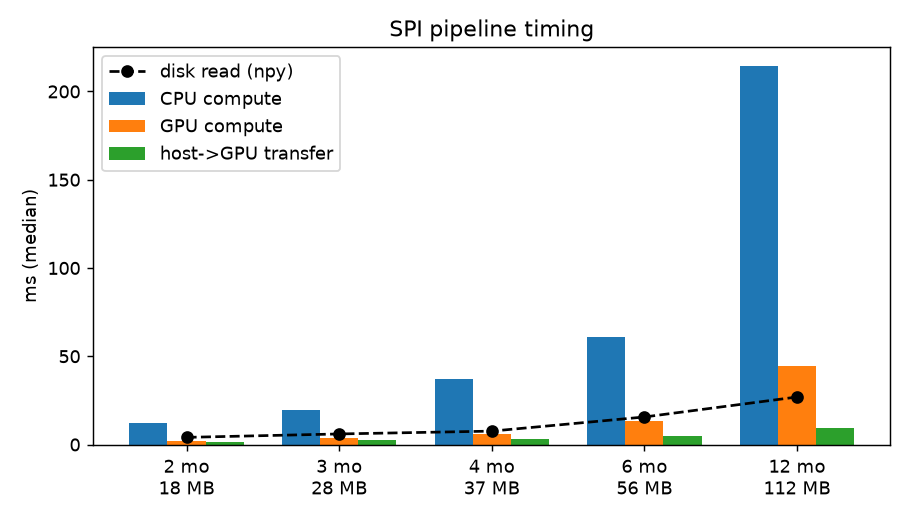
\includegraphics[width=0.62\linewidth]{timing.png}\caption{Tiempos por tama\~no de datos, en ms.}\end{figure}

\section{An\'alisis. Cuello de botella, Amdahl y 10 veces m\'as datos}
\textbf{Mover datos pesa casi tanto como calcular.} En la GPU, leer del disco (26.9 ms) y copiar a la GPU (9.3 ms) suman el 45\% del tiempo total del flujo (80.7 ms). El c\'omputo (44.5 ms) es el resto. En CPU la lectura es el 13\% del c\'omputo. Traer los datos desde el almac\'en remoto fue adem\'as la parte m\'as lenta e irregular del proyecto, pero depende de la red, as\'i que no entra en ning\'un c\'alculo de este informe.

\textbf{Ley de Amdahl.} La fracci\'on paralelizable del c\'omputo, todo salvo el conteo de d\'ias secos, es $f=98.6\%$ del tiempo en CPU. Si las partes paralelas se aceleran $S_p$ veces, el speedup es $S=1/((1-f)+f/S_p)$. Con el $S_p=3.5\times$ medido en las etapas, Amdahl predice 3.4$\times$, lo que coincide con lo observado. El flujo completo (lectura, copia y c\'omputo) mejora 3.0$\times$ y no 4.8$\times$, porque la lectura no se acelera y la copia es un costo extra que solo paga la GPU. Aun con c\'omputo gratis, el flujo completo no pasar\'ia de 6.7$\times$. El conteo de d\'ias secos tarda 1.9 ms en CPU y 5.6 ms en GPU, porque el ciclo lanza un \emph{kernel} por paso de tiempo y la latencia de lanzamiento supera al trabajo.

\textbf{Por qu\'e el speedup es modesto.} Es de 4 a 6 veces y no de 100. El problema es chico, cada celda hace poca aritm\'etica por byte le\'ido y las funciones especiales (\texttt{gammainc}, \texttt{ndtri}) pesan m\'as que las sumas. Con 10 veces m\'as datos todas las etapas escalan casi linealmente. La prueba de 9 veces m\'as celdas mantiene el speedup en 3.9$\times$, as\'i que la relaci\'on entre CPU y GPU no cambia con el tama\~no.

\section{Del benchmark al problema del MAGA}
El MAGA necesita actualizar el mapa de sequ\'ia cuando llegan datos nuevos y probar otras definiciones (otras escalas, otras resoluciones). Lo que importa es cu\'anto tarda una actualizaci\'on completa y cu\'antas variantes caben en una jornada. Con el costo por valor que medimos (lectura, copia y c\'omputo) proyectamos cuatro escenarios. Son \textbf{estimaciones lineales}, no mediciones, apoyadas en que la prueba de 9 veces m\'as celdas escal\'o casi linealmente.
\begin{table}[H]\centering\small
\begin{tabular}{llrrrr}\toprule & Escenario & Valores (mil millones) & GB (float32) & CPU & GPU \\\midrule
A & 12 meses, 0,25$^\circ$, 2 escalas (base medida) & 0.03 & 0.1 & 0.24 s & 0.08 s \\
B & 40 a\~nos, 0,25$^\circ$, 2 escalas & 1.12 & 4.5 & 10 s & 3 s \\
C & 40 a\~nos, 0,1$^\circ$ (ERA5-Land), 2 escalas & 6.99 & 28.0 & 60 s & 20 s \\
D & como C con 12 escalas (1 a 12 meses) & 6.99 & 28.0 & 6.0 min & 2.0 min \\
\\\bottomrule\end{tabular}\caption{Tiempo estimado de una actualizaci\'on completa del mapa.}\end{table}
La GPU no hace instant\'aneo el c\'alculo, lo acorta unas 3.0 veces. En el escenario D, un an\'alisis que en CPU toma 6.0 min toma 2.0 min en GPU. Esa es la diferencia entre dejar corriendo el trabajo y poder iterar sobre \'el. Como cada celda es independiente, los escenarios que no caben en la memoria de la GPU (C y D, cerca de 28 GB) se procesan por bloques de celdas sin cambiar el c\'odigo.

\section{Resultado e impacto para la industria}
\begin{figure}[H]\centering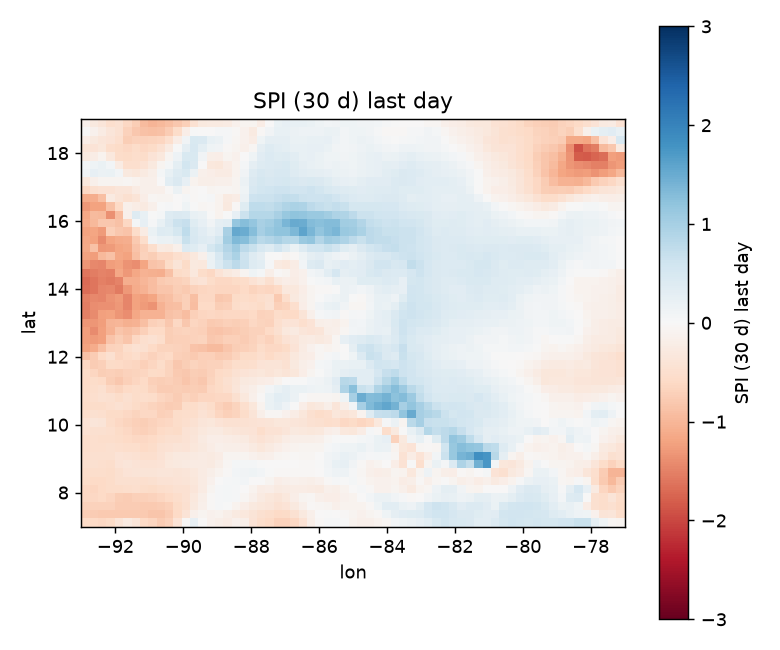
\includegraphics[width=0.46\linewidth]{spi30d_map.png}\hfill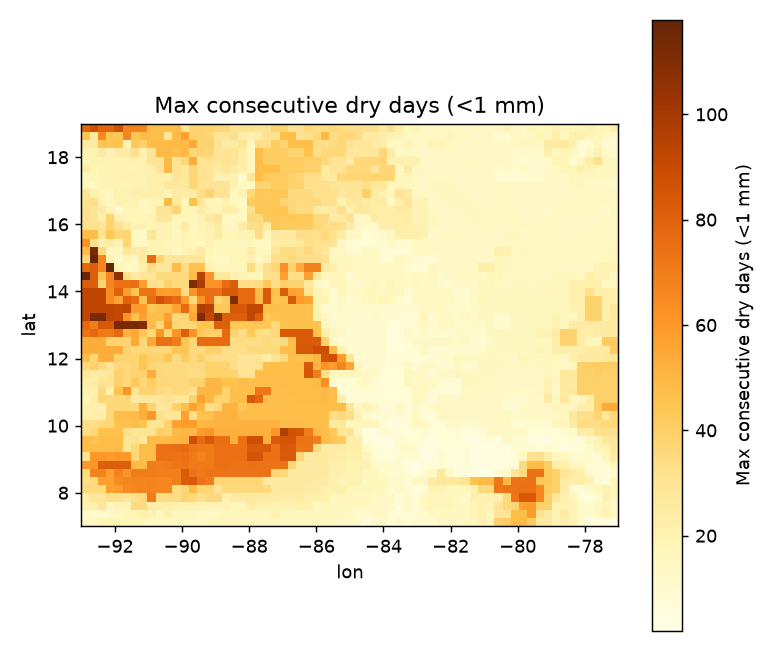
\includegraphics[width=0.46\linewidth]{dry_days_map.png}\caption{A la izquierda el SPI de 30 d\'ias el \'ultimo d\'ia de la serie, a la derecha el m\'aximo de d\'ias secos consecutivos.}\end{figure}
Con los datos ya en memoria, el mapa de SPI de toda Centroam\'erica se recalcula en una fracci\'on de segundo, as\'i que el MAGA puede cambiar la definici\'on de sequ\'ia y ver el mapa al instante. SPI-30d: 11\% de las celdas de Guatemala bajo $-1$ el último día (media -0.20). SPI-90d: 0\% de las celdas de Guatemala bajo $-1$ el último día (media +0.25).  El m\'aximo medio de d\'ias secos consecutivos en Guatemala es 31. Estas cifras no deben leerse como hallazgos de sequ\'ia, porque con tan pocos meses el ajuste gamma no es representativo. Lo que s\'i respalda la medici\'on es una recomendaci\'on operativa. Conviene invertir primero en la log\'istica de datos (guardar las series con partici\'on espacial o pedir subconjuntos regionales al servidor del CDS) y despu\'es en m\'as GPU.

\section{L\'imites}
\begin{itemize}
\item Solo 12 meses. No se midi\'o el escalamiento por a\~nos ni Guatemala contra Centroam\'erica, y la prueba de 10 veces es sint\'etica.
\item Una gamma por celda sobre todas sus ventanas (no una por mes del calendario), aproximaci\'on de Thom, escalas de 30 y 90 d\'ias y sin SPI de 6 meses.
\item Sin agregaci\'on municipal, porque no tenemos el shapefile, y sin validaci\'on contra a\~nos secos documentados, que requiere series largas.
\item Lectura de disco con cach\'e caliente. ERA5 es un rean\'alisis de $0{,}25^\circ$ y no son mediciones de estaci\'on.
\end{itemize}

\section{Reproducibilidad, uso de IA y fuentes}
\textbf{C\'odigo.} \url{https://github.com/TonitoMC/cuda-challenge-2}. Pasos, en orden, dentro de un entorno virtual con {\ttfamily\small numpy scipy xarray "zarr>=3" gcsfs cupy-cuda12x matplotlib pandas}. Se ejecutan {\ttfamily\small scripts/01\_download.py <a\~nos>, 01b\_clean.py, 02\_spi\_benchmark.py, 03\_plots.py y 04\_amdahl.py} (ver {\ttfamily\small README.md}). Se necesita una GPU NVIDIA con CUDA 12.

\textbf{Uso de IA.} El c\'odigo y el borrador de este informe se hicieron con ayuda de Claude Code (Anthropic). Los integrantes revisaron los resultados y pueden explicar cada parte.

\textbf{Fuentes.} Hersbach, H.\ et al.\ (2023), \emph{ERA5 hourly data on single levels from 1940 to present}, C3S CDS, doi:10.24381/cds.adbb2d47 (CC-BY 4.0). Copia ARCO-ERA5, Google Research y Cloud Public Datasets, \url{https://github.com/google-research/arco-era5}. McKee, Doesken y Kleist (1993), \emph{The relationship of drought frequency and duration to time scales}. Librer\'ias NumPy, SciPy, xarray, Zarr, CuPy, Matplotlib y pandas, y la documentaci\'on de NVIDIA CUDA, \url{https://docs.nvidia.com/cuda/}.
\end{document}
